\chapter{Theory of Operation} 
\label{theory}  
\section{Nuclear Polarization}
In the presence of a magnetic field, spin-\half{} nuclei tend to align themselves along the axis of the field.  The polarization of the ensemble of particles is defined by 

$$P=\frac{\uparrow-\downarrow}{\uparrow+\downarrow},$$

where ($\downarrow$, $\uparrow$) is the population of nuclei with $m_z$=(-\half,\half).
 \subsection{DNP}
Dynamic Nuclear Polarization (DNP) is a process of using microwave radiation to pump electron-proton pairs to higher energy (polarized) states.  The relaxation time for the electron is much shorter than that of the proton, so the proton remains polarized while the electron is able to be paired with other protons for polarization.

\begin{figure}
 \centering
 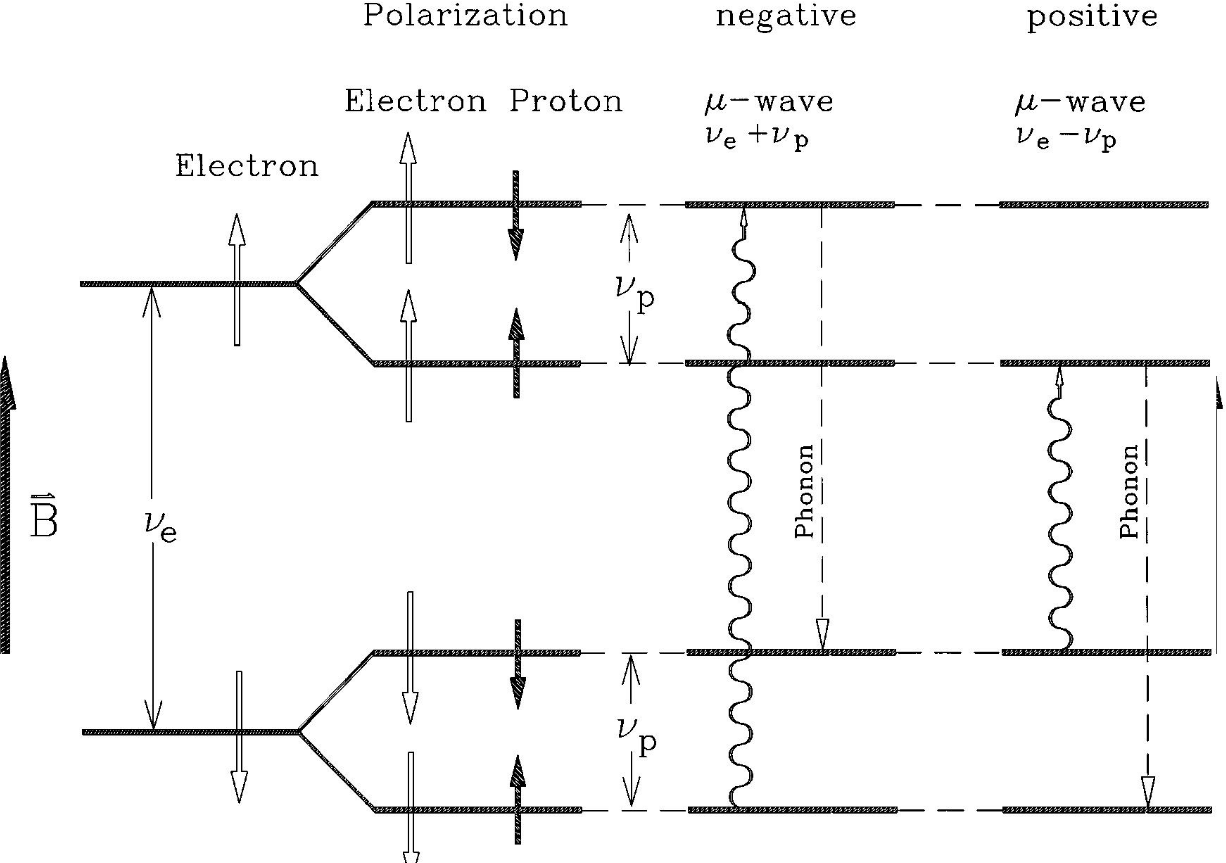
\includegraphics[scale=.25]{img/dnp.png}
 % dnp.png: 1226x863 pixel, 72dpi, 43.25x30.44 cm, bb=0 0 1226 863
 \caption{DNP diagram \cite{dnpdiagram}.  The white arrows are electron polarization and the black arrows are proton polarization.  Microwaves at a frequency difference $\nu_e\pm\nu_p$ flip the spins of both particles, and the electron's superior lattice coupling ensures it will flip back before the proton.}
 \label{fig:dnp-diagram}
\end{figure}


The microwave frequency used can be 
\section{NMR}

\section{Frozen Spin} 
 
\section{Dilution Refrigerator} 

